% Exercise 2.1 - Weekly Report
\documentclass[12pt]{article}
\usepackage{amsmath,graphicx}
\begin{document}
\section*{Summary}
This exercise implements and visualizes the Denoising Diffusion Probabilistic Model (DDPM) for image generation using a sprites dataset. The workflow includes forward diffusion (adding noise), reverse process (denoising), and model training. The code is modular, using configuration files for reproducibility.

\section*{Key Questions \& Answers}
\begin{itemize}
  \item \textbf{What is the purpose of the DDPM model?} DDPM is used for generating images by iteratively adding and removing noise, learning the reverse process via a neural network (UNet).
  \item \textbf{How is the diffusion process visualized?} The forward process is visualized by adding noise to images at various timesteps; the reverse process shows denoising using a pre-trained model.
  \item \textbf{What are the main challenges?} Ensuring correct device placement for tensors, managing paths for assets and models, and implementing the diffusion equations accurately.
\end{itemize}

\section*{Code Insights}

Main algorithms: Forward diffusion (q\_sample), reverse process (p\_sample\_loop), and UNet architecture for noise prediction. Results: Example sprites and diffusion parameters are visualized; model checkpoints and generated samples are saved. Challenges: Device mismatches (CPU/GPU), absolute path handling, and reproducible training via config files.

\section*{Visual Results}

\begin{figure}[h!]
  \centering
  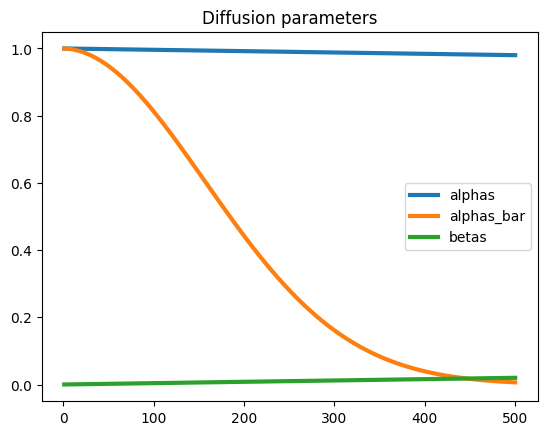
\includegraphics[width=0.45\textwidth]{../outputs/diffusion_params.png}
  \caption{Diffusion Parameters}
\end{figure}

\begin{figure}[h!]
  \centering
  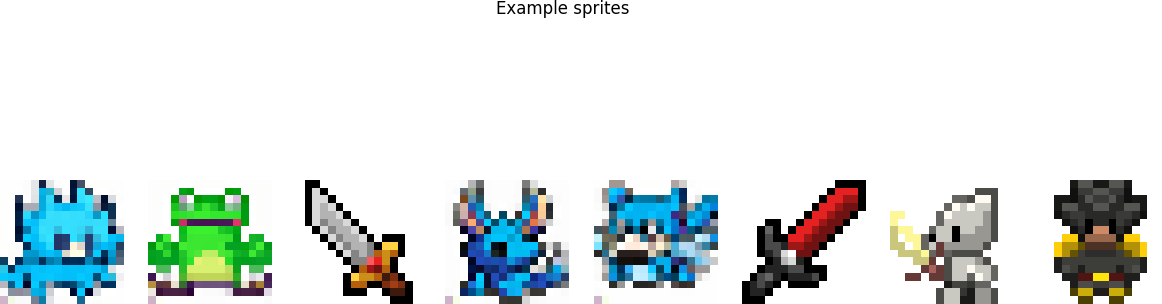
\includegraphics[width=0.45\textwidth]{../outputs/example.png}
  \caption{Example Sprites}
\end{figure}

\begin{figure}[h!]
  \centering
  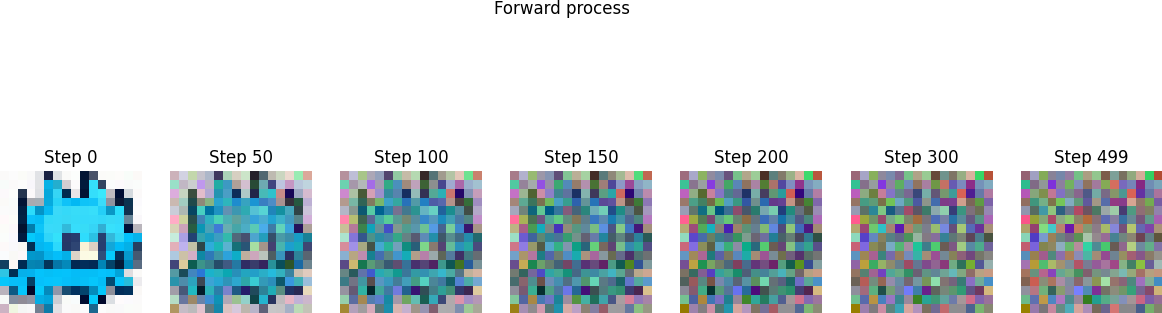
\includegraphics[width=0.45\textwidth]{../outputs/forward.png}
  \caption{Forward Process}
\end{figure}

\begin{figure}[h!]
  \centering
  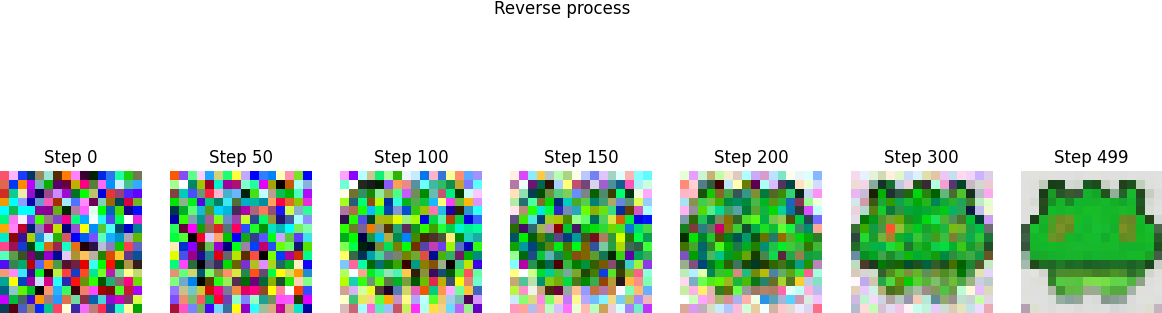
\includegraphics[width=0.45\textwidth]{../outputs/reverse.png}
  \caption{Reverse Process}
\end{figure}

\end{document}
